\section{Propagatore e invarianza di gauge}
Abbiamo detto che il propagatore fotonico è la funzione di Green dell'equazione del potenziale $A_\mu$
$$
\Box D_{\mu\nu}(x_1 - x_2) = g_{\mu\nu} \delta^4(x_1 - x_2)
$$
Siamo interessanti alla sua trasformata di Fourier
$$
\tilde{D}_{\mu\nu}(q) = \int D_{\mu\nu}(x) e^{-iq \cdot x} d^4x
$$
Nel dominio della variabile $q$ l'equazione diventa
$$
-q^2 \tilde{D}_{\mu\nu}(q) = g_{\mu\nu} \implies \tilde{D}_{\mu\nu}(q) = -\frac{g_{\mu\nu}}{q^2}
$$
Tuttavia sappiamo che l'equazione di $A_\mu$ non è la più generale. La forma che consideriamo presuppone il gauge di Lorentz $\partial^\mu A_\mu=0$. Ma nel caso generale senza fissare il gauge
$$
\Box A_\mu = 0 \implies \Box A_\mu - \partial_\mu \partial_\nu A^\nu = 0 \quad (\Box g_{\mu\nu} - \partial_\mu \partial_\nu) A^\nu = 0
$$
Verifichiamo che l'operatore $\Box g_{\mu\nu}-\partial_\mu\partial_\nu$ non ha un operatore inverso come avviene invece per l'equazione dell'onda precedente. Nello spazio dei momenti
$$
\hat{O} = -q^2 g_{\mu\nu} + q_\mu q_\nu
$$
Cerchiamo l'operatore inverso nella forma
$$
\hat{O}^{-1} = A g_{\mu\nu} + B q_\mu q_\nu
$$
Cerchiamo $A$ e $B$ tali che 
$$
\hat{O} \hat{O}^{-1} = 1
$$
Abbiamo
$$
\hat{O} \hat{O}^{-1} = (-q^2 g^{\mu\sigma} + q^\mu q^\sigma) (A g_{\sigma\nu} + B q_\sigma q_\nu) = \delta^\mu_\nu
$$
Sviluppando
$$
\hat{O} \hat{O}^{-1} = -q^2 A \delta^\mu_\nu - \cancel{B q^2 q^\mu q_\nu} + A q^\mu q_\nu + \cancel{B q^2 q^\mu q_\nu} = -q^2 A \delta^\mu_\nu + A q^\mu q_\nu = \delta^\mu_\nu
$$
Pertanto l'operatore non ha un inverso. Il problema viene risolto generalizzando l'equazione d'onda del potenziale $A_\mu$
$$
\Box A_\mu - \partial_\mu \partial_\nu A^\nu = 0 \quad \Longrightarrow \quad \Box A_\mu - \partial_\mu \partial_\nu A^\nu + \frac{1}{\xi} \partial_\mu \partial_\nu A^\nu = 0
$$
La generalizzazione equivale ad aggiungere un termine nella Lagrangiana
$$
\mathcal{L} = -\frac{1}{4} F_{\mu\nu} F^{\mu\nu} \quad \Longrightarrow \quad \mathcal{L}_\xi = -\frac{1}{4} F_{\mu\nu} F^{\mu\nu} - \frac{1}{2\xi}(\partial_\mu A^\mu)^2
$$
Verifichiamo che con questa generalizzazione l'inverso esiste ed è
$$
\tilde{D}_{\mu\nu}(q) = \frac{1}{q^2} \left[ -g_{\mu\nu} + \frac{(1 - \xi) q_\mu q_\nu}{q^2} \right]
$$
Utilizzando la stessa ipotesi
$$
O^{-1} = A g_{\sigma\nu} + B q_\sigma q_\nu
$$
Abbiamo
$$
\hat{O} \hat{O}^{-1} = \left( -q^2 g^{\mu\sigma} + (1 - \frac{1}{\xi}) q^\mu q^\sigma \right) (A g_{\sigma\nu} + B q_\sigma q_\nu) = \delta^\mu_\nu
$$
Sviluppando
$$
\hat{O} \hat{O}^{-1} = -q^2 A \delta^\mu_\nu - B q^2 q^\mu q_\nu + \left( 1 - \frac{1}{\xi} \right) A q^\mu q_\nu + \left( 1 - \frac{1}{\xi} \right) B q^2 q^\mu q_\nu
$$
Uguagliando rispettivamente a $1$ e a $0$ i coefficienti di $\delta_{\mu\nu}$ e $q_\mu q_\nu$
$$
-A q^2 = 1 \qquad \left( -B q^2 + \left( 1 - \frac{1}{\xi} \right) A + \left( 1 - \frac{1}{\xi} \right) B q^2 \right) q^\mu q_\nu = 0
$$
Otteniamo
$$
A = -\frac{1}{q^2} \text{ inserendo nella seconda eq. otteniamo }-B q^2 \frac{1}{\xi} = \frac{1}{q^2} \left( 1 - \frac{1}{\xi} \right)
$$
E infine
$$
B = - \frac{1}{q^2} \frac{\xi - 1}{q^2}
$$
Pertanto il propagatore è
$$
\tilde{D}_{\mu\nu}(q) = \frac{1}{q^2} \left[ -g_{\mu\nu} + \frac{(1 - \xi) q_\mu q_\nu}{q^2} \right]
$$
Il parametro $\xi$ permette di fissare il gauge. Il propagatore del fotone dipende dal gauge. Fra i valori più utilizzati:
\begin{itemize}
    \item Il gauge di Feynman $\xi=1$ che coincide con il gauge di Lorentz
    \item Il gauge di Landau $\xi=0$
\end{itemize}
Naturalmente il risultato fisico non può dipendere dal gauge. L'elemento di matrice deve essere indipendente da $\xi$. La conservazione della corrente elettromagnetica assicura che l'elemento di matrice sia indipendente dal gauge. Ricordiamo il risultato della $\mathfrak{M}_{fi}$
$$
\mathfrak{M}_{fi} = -i \frac{e^2}{2} \overline{u}_{p_3} \gamma^\mu u_{p_1} \tilde{D}_{\mu\nu}(q) \overline{u}_{p_4} \gamma^\nu u_{p_2} \qquad q = p_4 - p_2 = -(p_3 - p_1)
$$
Gli elementi di matrice delle correnti originavano da termini
$$
j^\mu(x) = \langle \mathbf{p}_4 | \hat{j}^\mu(x) | \mathbf{p}_2 \rangle = -e \overline{u}_{\mathbf{p}_4} \gamma^\mu u_{\mathbf{p}_2} e^{-i(p_4-p_2) \cdot x}
$$
Per l'invarianza di gauge della teoria questa corrente è conservata
$$
\partial_\mu j^\mu(x) = -e \overline{u}_{\mathbf{p}_4} \gamma^\mu u_{\mathbf{p}_2} \partial_\mu e^{-iq \cdot x} = i e \overline{u}_{\mathbf{p}_4} \gamma^\mu u_{\mathbf{p}_2} (p_4 - p_2)_\mu e^{-iq \cdot x} = i e \overline{u}_{\mathbf{p}_4} \gamma^\mu u_{\mathbf{p}_2} e^{-iq \cdot x} q_\mu
$$
Ricordiamo l'equazione di Dirac $\slashed{p}u_\mathbf{p}=mu_\mathbf{p}$
$$
\partial_\mu j^\mu(x) = i e \overline{u}_{\mathbf{p}_4} \gamma^\mu u_{\mathbf{p}_2} q_\mu e^{-iq \cdot x} = i e \overline{u}_{\mathbf{p}_4} (\slashed{p}_4 - \slashed{p}_2) u_{\mathbf{p}_2} e^{-iq \cdot x} = i e \overline{u}_{\mathbf{p}_4} (m - m) u_{\mathbf{p}_2} e^{-iq \cdot x} = 0
$$
Abbiamo pertanto verificato che per una corrente conservata $q_\mu j^\mu (x)=0$. Esaminiamo il propagatore nel generico gauge $\xi$.
$$
\tilde{D}_{\mu\nu}(q) = \frac{1}{q^2} \left[ -g_{\mu\nu} + \frac{(1 - \xi) q_\mu q_\nu}{q^2} \right]
$$
Osserviamo che se il propagatore è accoppiato a correnti conservate il termine gauge-dependent, che contiene $q_\mu q_\nu$, da un contributo nullo
$$
\mathfrak{M}_{fi} = - \frac{i}{2} j_{24}^\mu \tilde{D}_{\mu\nu}(q) j_{13}^\nu \qquad j_{24}^\mu = e \overline{u}_{\mathbf{p}_4} \gamma^\mu u_{\mathbf{p}_2} \qquad j_{13}^\mu = e \overline{u}_{\mathbf{p}_3} \gamma^\mu u_{\mathbf{p}_1}
$$
$$
\mathfrak{M}_{fi} = - \frac{i}{2} j_{24}^\mu \frac{g_{\mu\nu}}{q^2} j_{13}^\nu - \frac{i}{2} j_{24}^\mu \frac{1 - \xi}{q^4} q_\mu q_\nu j_{13}^\nu \quad \text{Gauge independent!}
$$
$$
j_{24}^\mu q_\mu = 0 \quad q_\nu j_{13}^\nu = 0 \qquad \mathfrak{M}_{fi} = - \frac{i}{2} j_{24}^\mu \frac{g_{\mu\nu}}{q^2} j_{13}^\nu
$$
\section{Teoria di Fermi del decadimento beta}
Nel decadimento $\beta^-$ un neutrone all'interno del nucleo si trasforma in un protone emettendo un elettrone e un antineutrino
$$
n\to pe^- \overline{\nu_e}
$$
All'interno del nucleo può avvenire un decadimento $\beta^+$ (proibito per un protone libero): la trasformazione di un protone in neutrone con l'emissione di un positrone e di un neutroni
$$
p\to pe^+ \nu_e
$$
La prima teoria soddisfacente del decadimento $\beta$ fu formulata da Enrico Fermi nel 1934. La storia della radioattività precedente al lavoro di Fermi a partire dalla scoperta di Bequerel è raccontata in un interessante articolo di A. Paris. Il decadimento $\beta$ è dovuto ad una forza molto debole, l'Interazione Debole. Nonostante sia poco intensa è molto importante e determina aspetti della nostra vita quotidiana. Ad esempio la velocità con cui procede la reazione di produzione del deuterio all'interno del sole:
$$
pp\to pne^+\nu \to D\gamma e^+ \nu
$$
Se avesse un tasso di produzione più elevato (intensità della forza maggiore) le stelle non avrebbero una vita longeva come la vediamo ora e la vita magari non avrebbe mai fatto tempo a crearsi!
\section{Decadimento beta del neutrone}
Enrico Fermi propose una teoria per il decadimento $\beta$ nel 1934. Fermi si ispirò all'interazione elettromagnetica di due particelle cariche che è interpretata come l'interazione di due correnti
\begin{figure}[h!]
    \centering
    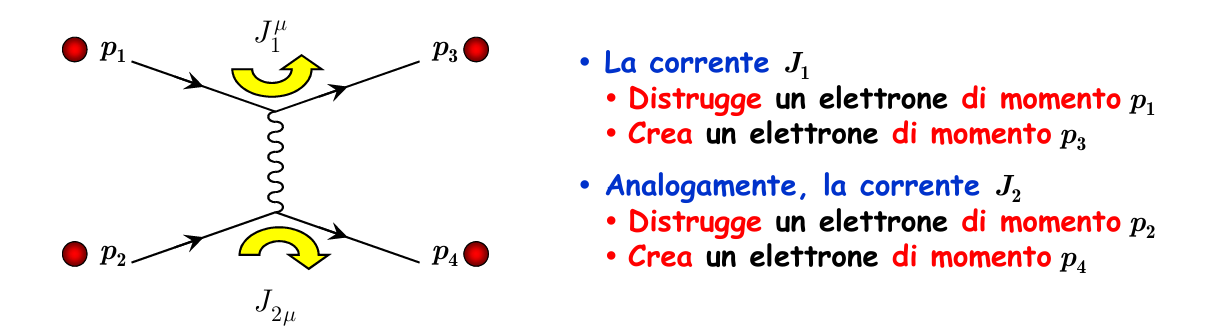
\includegraphics[width=0.9\textwidth]{Lezioni/Lezione 11/beta.png}
    \label{fig:beta}
\end{figure}
Le correnti introdotte sono costruite utilizzando gli operatori di campo $\hat{\psi}_e(x)$. Lungo la linea di una corrente ci sono delle grandezze fisiche che si conservano. In questo caso:
$$
J^\mu\sim \overline{\psi}_f\gamma^\mu\psi_i
$$
\begin{itemize}
    \item la carica elettrica ($\psi_i$ distrugge $-e$, $\psi_f$ crea $-e$)
    \item il numero fermionico
\end{itemize}
\begin{figure}[h!]
    \centering
    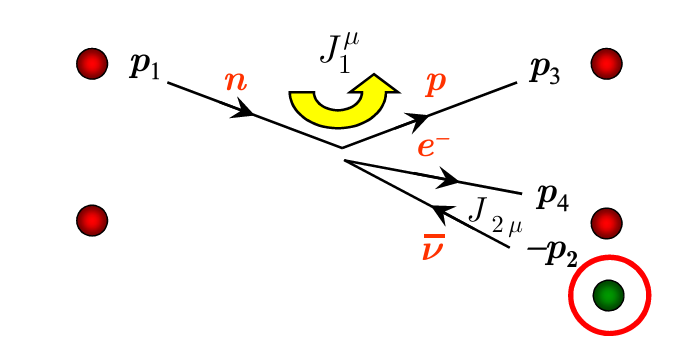
\includegraphics[width=0.5\textwidth]{Lezioni/Lezione 11/betaz.png}
    \label{fig:betaz}
\end{figure}
L'intuizione grandiosa di Fermi fu quello di mettere "insieme" neutrone e protone e neutrino ed elettrone. Poi fa questa associazione mettendo insieme neutrone e protone nella stessa corrente anche se effettivamente non c'è una conservazione di carica! Utilizzando questo modo di vedere anche per il decadimento $\beta$ per le due correnti hanno il seguente ruolo:
\begin{itemize}
    \item La corrente $J_1$ distrugge un neutrone $n$ di momento $p_1$ e crea un protone $p$ di momento $p_3$ (cambia il momento e cambia anche il tipo di particella).
    \item La corrente $J_2$ crea un elettrone $e^-$ di momento $p_4$ e distrugge un neutrino $\nu$ di momento $p_2$. Ovvero (guardando la figura) crea un antineutrino $\overline{\nu}$ di un momento $-p_2$
\end{itemize}
E quindi Fermi dice: va bene io posso creare una teoria in cui le correnti le scrivo come se fossero in elettromagnetismo prendendo la natura vettoriale della corrente e quindi $\gamma^\mu$. Si porta i campi delle particelle qui abbiamo 4 particelle di tipo diverso quindi 4 campi diversi! (Fermi ha avuto con se una decina di studenti che sono diventati a sua volta tutti premi Nobel. è fondamentale il maestro.) Fermi intuisce che c'è un numero che si conserva il numero barionico!
Cosa sostituisce il fotone? Fermi suppose una interazione di contatto
$$
\tilde{D}_{\mu\nu}(x_1, x_2) = g_{\mu\nu} \delta(x_1 - x_2) \qquad \mathcal{H}' \sim J^\mu_{pn}(x) g_{\mu\nu} J^\nu_{ev}(x)
$$
Oggi interpretiamo con lo scambio di un bosone carico e con massa $W^\pm$
\begin{figure}[h!]
    \centering
    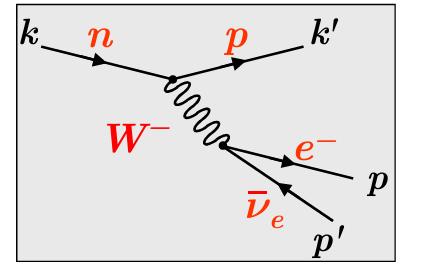
\includegraphics[width=0.4\textwidth]{Lezioni/Lezione 11/w.png}
    \label{fig:w}
\end{figure}
La prima è la corrente adronica che conserva il numero barionico
$$
N_n=1 \quad N_p=1 \quad 1=1
$$
Non conserva la carica elettrica. La seconda è la corrente leptonica e conserva il numero leptonico
$$
N_{e^-}=1 \quad N_{\overline{\nu}}=-1 \quad 0=1-1
$$
E anche questa non conserva la carica elettrica. Nel linguaggio della Teoria Quantistica dei Campi il decadimento viene descritto come la transizione da uno stato iniziale ad uno finale
$$
n \to p e^- \overline{\nu} \qquad |i\rangle = |n\rangle \qquad |f\rangle = |p e^- \overline{\nu}\rangle
$$
Sappiamo che la probabilità di transizione si calcola a partire dal corrispondente elemento della matrice $S$
$$
S_{if} = \langle f | \hat{S} | i \rangle
$$
L'operatore $S$ deve contenere gli opportuni operatori di campo in modo che l'elemento di matrice sia diverso da zero
$$
\hat{\psi} = \int \frac{d^3\mathbf{k}}{(2\pi)^3 \sqrt{2E_k}} \sum_\lambda (u_{k,\lambda} \hat{a}_{k,\lambda} e^{-ik\cdot x} + v_{k,\lambda} \hat{b}_{k,\lambda}^\dagger e^{+ik\cdot x})
$$
Dove $\hat{b}_{k,\lambda}^\dagger$ crea un antifermione e $\hat{a}_{k,\lambda}$ distrugge un fermione. Quindi nello stato iniziale viene distrutto:
\begin{itemize}
    \item Un neutrone $\to\psi_n$ perché è proprio $\psi$ che contiene l'operatore di distruzione di fermione
\end{itemize}
Nello stato finale vengono creati:
\begin{itemize}
    \item Un protone $\to\psi_p^\dagger$ abbiamo bisogno dell'operato di creazione che crei un fermione
    \item Un elettrone $\to\psi_e^\dagger$
    \item Un antineutrino $\to\psi_\nu$
\end{itemize}
Questi sono i quattro campi che dobbiamo mettere nella nostra teoria sottoforma di corrente. Fermi ipotizzò che l'interazione fosse descritta dalla densità Hamiltoniana
$$
\mathcal{H}' = G (\overline{\psi}_p \gamma^\mu \psi_n) (\overline{\psi}_e \gamma_\mu \psi_\nu)
$$
Ricordando che tutti i campi sono calcolati nello stesso punto spazio-temporale $x$. La transizione è pertanto dovuta a una interazione di contatto e puntiforme. Il termine di interazione da aggiungere alla Lagrangiana è $\mathcal{L}'=-\mathcal{H}'$. Qui il vertice ha quattro fermioni e messi nello stesso punto. Quindi stesso punto dello spaziotempo con quattro rami. A differenza del caso dell'elettromagnetismo in cui in un vertice ho tre particelle: due fermioni e un fotone.
La stessa Hamiltoniana (completa con un ulteriore termine hermitiano coniugato) può descrivere altre interazioni ad esempio
Dove:
$$
\mathcal{H}' = G (\overline{\psi}_p \gamma^\mu \psi_n) (\overline{\psi}_e \gamma_\mu \psi_\nu) + h.c.
$$
\begin{itemize}
    \item Distrugge un neutrino
    \item Distrugge un neutrone
    \item Crea un protone
    \item Crea un elettrone
\end{itemize}
Quali altre relazioni descrive l'Hamiltoniana? E in particolare, il termine h.c.

Nota curiosa: La teoria di Fermi fu pubblicata in Z. Physik nel 1934. L'articolo fu prima sottoposto per la pubblicazione a Nature che lo rifiutò con la seguente motivazione "...because it contains speculations too remote from reality to be of interest to the reader"
\subsection{La costante G}
Questa costante ci dice praticamente quanto è intensa l'interazione. C'è qualcosa di anomalo in quanto notiamo per finire le dimensioni della costante $G$. La densità Hamiltoniana $\mathcal{H}'$ deve avere le dimensioni di una densità di energia: $[\mathcal{H}']=ML^{-3}=M^4$. Alternativamente l'integrale $\int\mathcal{L'}d^4x$ è un'azione e nelle unità di misura naturali deve essere adimensionale: $[\mathcal{L}']L^4=[\mathcal{L}']M^{-4}\to[\mathcal{L}']=M^4$. Le dimensioni del campo $\psi$ si possono dedurre dal termine cinetico della lagrangiana $i\overline{\psi}\slashed{\partial}\psi$ da cui $[\psi]^2L^{-1}=[\psi]^2M^1=M^4$ ed infine $[\psi]^2=M^3$, $[\psi]=M^{3/2}$. Dalla rappresentazione integrale
$$
\hat{\psi} = \int \frac{d^3\mathbf{k}}{(2\pi)^3 \sqrt{2E_k}} \sum_\lambda (u_{k,\lambda} \hat{a}_{k,\lambda} e^{-ik\cdot x} + v_{k,\lambda} \hat{b}_{k,\lambda}^\dagger e^{+ik\cdot x})
$$
Inoltre $[u]=M^{1/2}$ e $[a]=[b]=M^{-3/2}$
$$
u,v \sim \sqrt{E} \qquad \{\hat{a}_k, \hat{a}_k^\dagger\} \sim \delta(k-k')
$$
Pertanto di nuovo $[\psi]=M^{3/2}$. La dimensione della costante $G$ risulta quindi 
$$
[G] [\psi]^4 = M^4 \to [G][M^{3/2}]^4 = M^4 = [G][M]^6
$$
da cui 
$$
[G] = M^{-2}
$$
Notare che nel caso della interazione elettromagnetica la costante di accoppiamento $\alpha$ è adimensionale
$$
\alpha = \frac{e^2}{4\pi\epsilon_0 \hbar c} \approx \frac{1}{137}
$$
Nel caso dell'interazione elettromagnetica la dimensione $M^{-2}$ necessaria per rendere adimensionale l'ampiezza è introdotta dal propagatore ($q^2$) quindi questo risulta un ottimo indizio sul fatto che manca il propagatore.
\subsection{L'elemento di matrice}
Impostiamo adess il calcolo dell'elemento di matrice. Abbiamo bisogno di esprimere gli stati dello spazio di Fock utilizzando gli opportuni operatori di creazione 
$$ 
|n\rangle = \hat{a}_{pn}^\dagger |0\rangle \quad |pe^-\overline{\nu}\rangle = \hat{a}_{pp}^\dagger \hat{a}_{pe}^\dagger \hat{b}_{p\nu}^\dagger |0\rangle \quad \langle pe^-\overline{\nu}| = \langle 0 | \hat{a}_{pp} \hat{a}_{pe} \hat{b}_{p\nu}
$$
Per semplificare la notazione abbiamo posto:
$$
pp=p_p; \quad pn=p_n; \quad pe=p_e; \quad p\nu=p_\nu
$$
Inoltre è sottointeso che $a_{pp}^\dagger \equiv \sqrt{2E_{pp}} a_{pp}^\dagger $(li inseriremo alla fine). Al primo ordine dello sviluppo perturbativo l'ampiezza della transizione è data dall'elemento di matrice dell'Hamiltoniana $H'$ fra stato inziale e stato finale
$$
\mathcal{A}_{fi} = -i \int dt \langle pe^-\overline{\nu} | H'_I | n \rangle = -i \int d^4x \langle 0 | \hat{a}_{pp} \hat{a}_{pe} \hat{b}_{p\nu} \hat{\mathcal{H}}'_I \hat{a}_{pn}^\dagger |0\rangle \quad H'_I = \int \mathcal{H}'_I d^3x
$$
Per calcolare esplicitamente l'elemento di matrice si introduce l'espressione della densità Hamiltoniana
$$
\mathcal{H}'_I = G (\overline{\psi}_p \gamma^\mu \psi_n) (\overline{\psi}_e \gamma_\mu \psi_\nu)
$$
Si sostituiscono gli operatore di campo nella densità Hamiltoniana con le rappresentazioni integrali
$$
\hat{\psi} = \int \frac{d^3\mathbf{k}}{(2\pi)^3 \sqrt{2E_k}} \sum_\lambda (u_{k,\lambda} \hat{a}_{k,\lambda} e^{-ik\cdot x} + v_{k,\lambda} \hat{b}_{k,\lambda}^\dagger e^{+ik\cdot x})
$$
Otteniamo pertanto
$$
\mathcal{A}_{fi} = -iG \int d^4x \langle 0 | \hat{a}_{pp} \hat{a}_{pe} \hat{b}_{p\nu} (\overline{\psi}_p \gamma^\mu \psi_n) (\overline{\psi}_e \gamma_\mu \psi_\nu) \hat{a}_{pn}^\dagger |0\rangle
$$
Ricordiamo che tutti i campi sono calcolati nello stesso punto: $\psi(x)$ e ricordiamo inoltre che lo spazio di Fock del nostro sistema è un prodotto tensoriale di stati di singola particella
$$
|pe^-\overline{\nu}\rangle = \hat{a}_{pp}^\dagger \hat{a}_{pe}^\dagger \hat{b}_{p\nu}^\dagger |0\rangle \quad |0\rangle = |0\rangle_p \otimes |0\rangle_n \otimes |0\rangle_e \otimes |0\rangle_\nu \quad |pe^-\overline{\nu}\rangle = \hat{a}_{pp}^\dagger |0\rangle \otimes \hat{a}_{pe}^\dagger |0\rangle \otimes \hat{b}_{p\nu}^\dagger |0\rangle_n
$$
Possiamo pertanto riscrivere l'elemento di mtrice come
$$
\mathcal{A}_{fi} = -iG \int d^4x \langle 0 | \hat{a}_{pp} \overline{\psi}_p \gamma^\mu \psi_n \hat{a}_{pn}^\dagger |0\rangle \langle 0 | \hat{a}_{pe} \hat{b}_{p\nu} \overline{\psi}_e \gamma_\mu \psi_\nu |0\rangle
$$
Considerimo il termine leptonico
$$
\langle 0 | \hat{a}_{pe} \hat{b}_{p\nu} \overline{\psi}_e \gamma_\mu \psi_\nu |0\rangle = 
$$
$$
= \int \frac{d^3\mathbf{k}_e}{(2\pi)^3 \sqrt{2E_e}} \frac{d^3\mathbf{k}_\nu}{(2\pi)^3 \sqrt{2E_\nu}} \langle 0 | \hat{a}_{pe} \hat{b}_{p\nu} (\overline{u}_{k_e} \hat{a}_{k_e} e^{+ik_e \cdot x} + \overline{v}_{k_e} \hat{b}_{k_e} e^{-ik_e \cdot x}) \gamma_\mu (u_{k_\nu} \hat{a}_{k_\nu} e^{-ik_\nu \cdot x} + v_{k_\nu} \hat{b}_{k_\nu}^\dagger e^{+ik_\nu \cdot x}) |0\rangle
$$
$$
= \int \frac{d^3\mathbf{k}_e}{(2\pi)^3 \sqrt{2E_e}} \frac{d^3\mathbf{k}_\nu}{(2\pi)^3 \sqrt{2E_\nu}} \langle 0 | \hat{\mathcal{O}}_l | 0 \rangle
$$
L'ultima uguaglinza definisce l'operatore $\overline{\mathcal{O}}_l$. Dopo vari conti non richiesti si ottiene infine
$$
\langle e\overline{\nu} | \overline{\psi}_e \gamma_\mu \psi_\nu | 0 \rangle = \langle 0 | \hat{a}_{pe} \hat{b}_{p\nu} \overline{\psi}_e \gamma_\mu \psi_\nu | 0 \rangle = \overline{u}_{p_e} \gamma_\mu v_{p_\nu} e^{i(p_e + p_\nu) \cdot x}
$$
$$
\langle p | \overline{\psi}_p \gamma^\mu \psi_n | n \rangle = \langle 0 | \hat{a}_{pp} \overline{\psi}_p \gamma^\mu \psi_n \hat{a}_{pn}^\dagger | 0 \rangle = \overline{u}_{p_p} \gamma^\mu u_{p_n} e^{i(p_p - p_n) \cdot x}
$$
Ricordiamo inoltre l'espressione per l'ampiezza di transizione
$$
\mathcal{A}_{fi} = -iG \int d^4x \langle 0 | \hat{a}_{pp} \overline{\psi}_p \gamma^\mu \psi_n \hat{a}_{pn}^\dagger |0\rangle \langle 0 | \hat{a}_{pe} \hat{b}_{p\nu} \overline{\psi}_e \gamma_\mu \psi_\nu |0\rangle
$$
Inserendo i risultati trovati si trova
$$
\mathcal{A}_{fi} = -iG \overline{u}_{p_p} \gamma^\mu u_{p_n} \overline{u}_{p_e} \gamma_\mu v_{p_\nu} \int d^4x e^{i(p_p - p_n) \cdot x} e^{i(p_e + p_\nu) \cdot x}
$$
$$
\mathcal{A}_{fi} = -iG \overline{u}_{p_p} \gamma^\mu u_{p_n} \overline{u}_{p_e} \gamma_\mu v_{p_\nu} (2\pi)^4 \delta^4(p_n - p_p - p_\nu - p_e)
$$
L'ampiezza invariante è
$$
\mathcal{A}_{fi} = \mathfrak{M}_{fi} (2\pi)^4 \delta^4(\dots)\qquad \mathfrak{M}_{fi} = -iG \overline{u}_{p_p} \gamma^\mu u_{p_n} \overline{u}_{p_e} \gamma_\mu v_{p_\nu}
$$
Osserviamo che l'ampiezza non contiene il propagatore
$$
\mathfrak{M}_{fi} = -iG \overline{u}_p \gamma^\mu u_n \overline{u}_{p_e} \gamma_\mu v_{p_\nu}
$$
Al suo posto c'è la costante dimensionale $G$. In futuro le ampiezze potranno essere scritte utilizzando regole e diagrammi di Feynman senza rifare tutto il calcolo con la teoria dei campi. Le regole di Feynman possono essere dedotte osservando il termine della Lagrangiana relatico alla interazione fra i campi. Ricordando che $\mathcal{H'}=-\mathcal{L'}$
$$
\mathcal{L}' = -G(\overline{\psi}_p \gamma^\mu \psi_n)(\overline{\psi}_e \gamma_\mu \psi_\nu) + h.c.
$$
Al primo ordine corrispondono i diagrammi con un solo vertice e $4$ linee
\begin{figure}[h!]
    \centering
    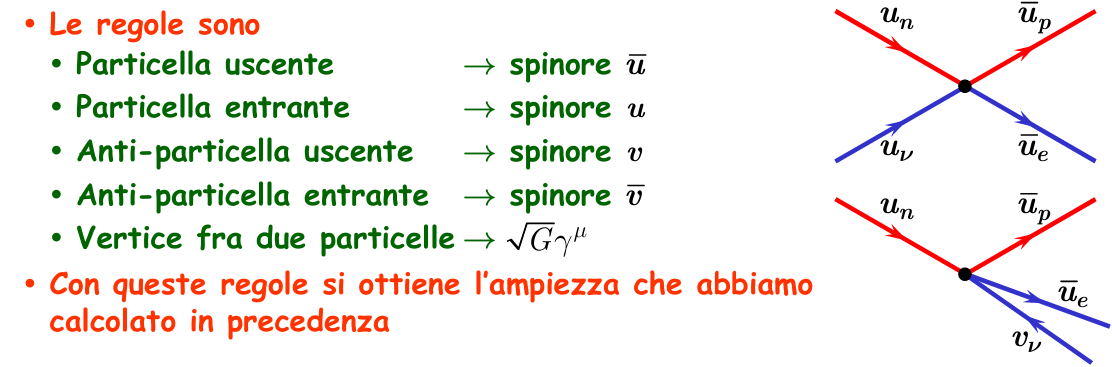
\includegraphics[width=0.8\textwidth]{Lezioni/Lezione 11/ui.png}
    \label{fig:ui}
\end{figure}
\section{Cinematica decadimento in tre corpi}
Da ora in poi $c=1$. Variabili invarianti nel decadimento 
\begin{figure}[h!]
    \centering
    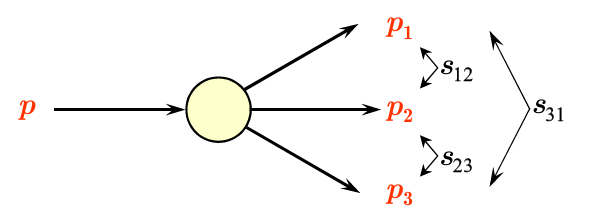
\includegraphics[width=0.8\textwidth]{Lezioni/Lezione 11/io.png}
    \label{fig:io}
\end{figure}
La conservazione del $4-$impulso
$$
p=p_1+p_2+p_3
$$
Sono convenienti le seguenti variabili invarianti (utuali in tutti i sistemi di riferimento inerziale)
$$
s_{12} = (p_1 + p_2)^2 = (p - p_3)^2 \quad s_{23} = (p_2 + p_3)^2 = (p - p_1)^2 \quad s_{31} = (p_3 + p_1)^2 = (p - p_2)^2
$$
la variabile $s_{ij}$ è anche detta massa invariante (al quadrato) del sistema composto dalle $2$ particelle $i$ e $j$. Inoltre
$$
s = p^2 = (p_1 + p_2 + p_3)^2 = m^2
$$
E si verifica facilmente che
$$
s_{12} + s_{23} + s_{31} = m^2 + m_1^2 + m_2^2 + m_3^2
$$
Nel sistema di riferimento in cui la particella $p$ è a riposo
$$
p=(m,\mathbf{0}) \qquad s=p^2=m^2
$$
La somma dei momenti dei prodotti di decaimento è nulla, i tre momenti giacciono su un piano. Quindi ho 
\begin{itemize}
    \item 3 impulsi $\times$ 3 componenti $=9$
    \item 4 equazioni $p=p_1+p_2+p_3$
    \item 1 angolo inessenziale di rotazione nel piano
    \item 2 angoli inessenziali di orientamento nel piano
\end{itemize}
Quindi le variabili indipendenti sono $9-4-1-2=2$. Si possono quindi utilizzare una coppia di $s_{ij}$ qualsiasi. Si possono definire energie e momenti delle $3$ particelle nello stato finale (nel sistema di riposo della particella $p$) in funzione di variabili invarianti
$$
s_{23} = (p - p_1)^2 = m^2 + m_1^2 - 2mE_1 \qquad E_1 = \frac{m^2 + m_1^2 - s_{23}}{2m}
$$
Questa è la stessa formula di una particella di massa $m$ che decade in una particella di massa $m_1$ e una di massa $m_{23}=\sqrt{s_{23}}$. Il momento della particella
$$
|\mathbf{p}_1|^2 = E_1^2 - m_1^2 \qquad |\mathbf{p}_1| = \frac{\lambda^{1/2}(m^2, m_1^2, s_{23})}{2m}
$$
La funzione $\lambda$ è
$$
\lambda(x, y, z) = (x - y - z)^2 - 4yz
$$
Analogamente si trovano le relazioni per le altre particelle:

\begin{align*}
E_1 &= \frac{m^2 + m_1^2 - s_{23}}{2m} & |\mathbf{p}_1| &= \frac{\lambda^{1/2}(m^2, m_1^2, s_{23})}{2m} \\
E_2 &= \frac{m^2 + m_2^2 - s_{31}}{2m} & |\mathbf{p}_2| &= \frac{\lambda^{1/2}(m^2, m_2^2, s_{31})}{2m} \\
E_3 &= \frac{m^2 + m_3^2 - s_{12}}{2m} & |\mathbf{p}_3| &= \frac{\lambda^{1/2}(m^2, m_3^2, s_{12})}{2m}
\end{align*}
Per il calcolo degli angoli si può procedere in modo analogo
$$
s_{23} = (p_2 + p_3)^2
$$
$$
s_{23} = m_2^2 + m_3^2 + 2E_2 E_3 - 2 |\mathbf{p}_2| |\mathbf{p}_3| \cos\theta_{23}
$$
$$
\cos\theta_{23} = \frac{-s_{23} + m_2^2 + m_3^2 + 2E_2 E_3}{2 |\mathbf{p}_2| |\mathbf{p}_3|}
$$
$$
\cos\theta_{23} = \frac{-s_{23} + m_2^2 + m_3^2 + 2E_2 E_3}{\lambda^{1/2}(m^2, m_2^2, s_{31}) \lambda^{1/2}(m^2, m_3^2, s_{12}) \frac{1}{2m^2}}
$$
$$
\cos\theta_{23} = \frac{2m^2(m_2^2 + m_3^2 - s_{23}) + 4m^2 E_2 E_3}{\lambda^{1/2}(m^2, m_2^2, s_{31}) \lambda^{1/2}(m^2, m_3^2, s_{12})}
$$
$$
\cos\theta_{23} = \frac{2m^2(m_2^2 + m_3^2 - s_{23}) + (m^2 + m_2^2 - s_{31})(m^2 + m_3^2 - s_{12})}{\lambda^{1/2}(m^2, m_2^2, s_{31}) \lambda^{1/2}(m^2, m_3^2, s_{12})}
$$
Pertanto, una volta fissate due variabili $s_{ij}$, tutte le altre grandezze cinematiche sono determinate
\section{Regione fisica del decadimento}
Una volta scelte due variabili $s_{ij}$ per descrivere lo stato finale occorre definire la regione fisica che le due variabili possono assumere
\begin{figure}[h!]
    \centering
    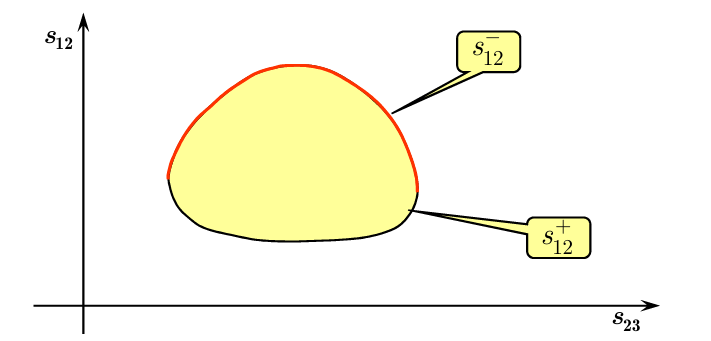
\includegraphics[width=0.8\textwidth]{Lezioni/Lezione 11/s.png}
    \label{fig:s}
\end{figure}
Scegliamo, ad esempio, $s_{12}$ e $s_{23}$ come variabili indipendenti. L'equazione che definisce la frontiera sul piano $s_{12} -s_{23}$ è definita da
$$
s_{12}^\pm = m_1^2 + m_2^2 - \frac{1}{2s_{23}} [ (s_{23} - m^2 + m_1^2)(s_{23} + m_2^2 - m_3^2) \mp \lambda^{1/2}(s_{23}, m_2^2, m_1^2) \lambda^{1/2}(s_{23}, m_2^2, m_3^2) ]
$$
La regione di variabilità di $s_{23}$ si può trovare imponendo la realtà delle radici
$$
\lambda(s_{23}, m_1^2, m_2^2) \ge 0 \qquad \lambda(s_{23}, m_2^2, m_3^2) \ge 0
$$
Oppure attraverso ragionamenti fisici fatti a Fidica delle Particelle quando abbiamo studiato i Dalitz Plot.
\section{Cinematica decadimento beta del neutrone}
Facendo riferimento alla figura
\begin{figure}[h!]
    \centering
    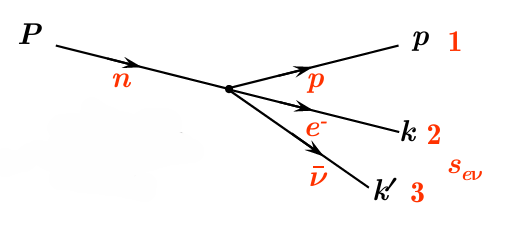
\includegraphics[width=0.8\textwidth]{Lezioni/Lezione 11/yyy.png}
    \label{fig:yyy}
\end{figure}
Le energie sono date da
$$
E_p = \frac{m_n^2 + m_p^2 - s_{e\nu}}{2m_n} \qquad E_e = \frac{m_n^2 + m_e^2 - s_{\nu p}}{2m_n} \qquad E_\nu = \frac{m_n^2 - s_{pe}}{2m_n}
$$
Abbiamo appena visto che
$$
(m_2 + m_3)^2 \le s_{23} \le (m_2 - m_1)^2 \qquad m_e^2 \le s_{e\nu} \le (m_n - m_p)^2
$$
Dalla equazione per $E_p$ possiamo ricavare
$$
s_{e\nu} = m_n^2 + m_p^2 - 2m_n E_p \qquad m_n^2 + m_p^2 - 2m_n E_p \ge m_e^2 \qquad \frac{m_n^2 + m_p^2 - m_e^2}{2m_n} \ge E_p
$$
L'energia cinetica del protone è
$$
T_p = E_p - m_p \qquad \frac{m_n^2 + m_p^2 - m_e^2}{2m_n} - m_p \ge T_p \qquad\frac{(m_n - m_p)^2 - m_e^2}{2m_n} \ge T_p
$$
Analogamente si ottiene
$$
E_e \le \frac{m_n^2 - m_p^2 + m_e^2}{2m_n}
$$
Utilizzando i valori noti delle masse
\begin{itemize}
    \item $m_e=0.511\,\unit{MeV}$
    \item $m_n=939.560\,\unit{MeV}$
    \item $m_p=938.270\,\unit{MeV}$
\end{itemize}
Si ottiene in definitica $E_e\le1.29\,\unit{MeV}$. Vediamo che, almeno vicino al limite della regione permessa, l'elettrone può raggiungere velocità realtivistiche. Analogamente, il limite superiore alla energia cinetica del protone
$$
T_p \le \frac{(m_n - m_p)^2 - m_e^2}{2m_n} = 0.75 \, \text{KeV}
$$
Calcoliamo il limite supriore alla velocità del protone
$$
\beta_p = \sqrt{\frac{2T_p}{m_p}} \le \sqrt{\frac{(m_n - m_p)^2 - m_e^2}{m_p m_n}} \approx \frac{\Delta m}{m_p} \approx \frac{1.29}{938} \approx 1.4 \cdot 10^{-3}
$$
Il protone è sempre non relativistico. 

Riassumento:
\begin{itemize}
    \item Nel sistema di laboratorio l'elettrone può raggiungere velocità relativistiche.
    \item Il neutrino, che assumiamo avere massa nulla, ha sempre velocità relativistiche ($\beta_\nu=1$).
    \item Il neutrone è a riposo
    \item Il protone ha velocità non relativistiche
\end{itemize}
Per i leptoni è pertanto indispensabile utilizzare una teoria relativistica (utilizzeremo gli spinori quadridimensionali). Per il protone e per il neutrone è sufficiente un'approssimazione non relativistica (utilizzeremo gli spinori bidimensionali di Pauli). Per un nucleo valgono gli stessi argomenti!